\subsection{选取最好的战舰}
\begin{formal}
    {\cuhei 问题描述:}

    明天,人类舰队就要迎接三体舰队的探测器——水滴了,作为增援未来部队的你(章北海)刚从“冬眠”中苏醒,就立刻思考起了保留人类文明火种的重大计划,逃亡!
为了增加逃亡的成功率,你用1秒钟快速了解了所有战舰的历史表现数据(速度、火力)和目前物资储备(食物、燃料),并选出了一艘最合适的战舰。
\end{formal}
\begin{formal}
    {\cuhei 输入要求:}

    \begin{enumerate}
        \item 输入包含若干张表,每一张表表示部分战舰在某个方面的数据表中有若干键值对,键为战舰的名字,值为该战舰的一项数据(均为浮点数)。输入战舰顺序不确定
        \item 可以认为每一张表都表示不同的数据(即不会有两张表都表示战舰的加速度),且同一张表中一艘战舰只会出现一次,且每张表中都包含所有战舰的这一个数据(即不会有战舰缺某项数据)
        \item 每一项数据都有一个权值,表示你认为这项数据的重要程度。假设表i中记录战舰j的数据为tij,表的权值为wi,那么这艘战舰的总分数计算方法为cj=t1j*w1+t2j*w2+ ... + tnj*wn
        \item 你可以自己假设表格的输入格式细节
        \item 要求使用字典树作为基础数据结构
    \end{enumerate}
\end{formal}
\begin{formal}
    {\cuhei 输出要求:}

    \begin{enumerate}
        \item 输出一张大表,表的行为战舰名字,列为不同的数据(乘上权值),并打印总分
        \item 要求所有战舰按总分从大到小排列,对列的顺序没有要求
        \item 你可以自己假设输出格式的细节
    \end{enumerate}
\end{formal}
\subsubsection{问题分析与解决思路}
本题在输入输出方面给了较大的自由度,唯一的限制是使用字典树。这里之所以有必要使用字典树,
是因为每张表格的战舰输入顺序不同,导致每输入一个数值,都需要先查找到对应战舰的存储位置,不能根据输入次序直接随机存储,
从而不适合使用线性表。

本题不要求在最后的输出中包含表的权重,因此可以在处理表的输入时,便将加权的分数计算出来,后续便不再需要表的权重。

由于字典树的结构无法改动,所以无法直接在它上面进行排序,所以在处理完所有表的输入后,还需要将存储的各个战舰的信息从
字典树导出到数组中,以便后续的排序操作。

为了提高效率,用于排序的数组元素中,除了用于排序的key之外,便只有指向字典树结点的指针。
\subsubsection{数据结构设计}
\begin{lstlisting}[name=Q1]
string val_name[MAXDATAN];//存储各属性的名称
class DT
{
    DT* children[MAXN];//存储指向孩子结点的指针
    prop* data;//存储得分
    char key;//该结点对应的字符
    State state;//是否为某字符串的结尾
    string name;//若该结点为某字符串的结尾,则存储该字符串
};
struct prop
{
    double val[MAXDATAN];//存储各数据的数值
    double sum;//总分数
};
enum State
{
    mid = 0,
    end ,//是某个字符串的结尾
};
struct ElemType
{
    DT* data;//字典树中的一个结点
    double key;//该节点对应的总分数,排序依据
};
struct Array//用于排序
{
    int size;//方便向末端添加元素
    ElemType ships[MAXN];
}
\end{lstlisting}
\subsubsection{功能描述}
\begin{function}
    \SetKwFunction{build}{Build-Tree}
    \SetKwFunction{traverse}{Traverse-Tree}
    \SetKwFunction{add}{Add-Ship}
    \SetKwFunction{quick}{Quick-Sort}
    \SetKw{in}{in}
    \KwIn{空字典树T,数据表格tables}
    \KwOut{按总得分降序排列的数组ships}
    first = 1\;
    \ForEach{table \in tables}
    {
        \eIf{first ==1}
        {
            first = 0\;
            \build(T,table)\;
        }
        {
            \add(T,table)\;
        }
    }
    ships = \traverse(T)\;
    \quick(ships)\;
    \KwRet{ships}\;
    \caption{Sort-Ship(T)}
\end{function}
\begin{function}[H]
    \SetKw{in}{in}
    打印val-name\tcp*[h]{各属性名称}\;
    \ForEach{ship \in ships}
    {
        打印ship $\rightarrow$data $\rightarrow$name\;
        打印ship $\rightarrow$data $\rightarrow$val\;
        打印ship $\rightarrow$data $\rightarrow$sum\;
    }
    \caption{Print-Ship(ships)}
\end{function}
\begin{function}
    \KwIn{空字典树T,表格table}
    \SetKw{NULL}{NULL}
    \ForEach(\tcp*[h]{遍历每只战舰}){table.record}
    {
        p = T\;
        \For{i = 1 \KwTo record.name.length}
        {
            j = 1\;
            \lWhile{p$\rightarrow$ children[j]$\neq$\NULL and p$\rightarrow$children[j].key $\neq$record.name[i]}{j+=1}
            \tcp*[h]{寻找子节点}\;
            \If(\tcp*[h]{未找到}){p $\rightarrow$ children[j]==\NULL}
            {
                新建结点 newNode\tcp*[h]{state为mid,key为record.name[i],data置零}\;
                p $\rightarrow$children[j] = newNode\;
            }
            p = record.children[j]\tcp*[h]{更新指针}\;         
            \If(\tcp*[h]{标记为字符串结尾}){i == record.name.length}
            {
            p $\rightarrow$ state = end\;
            更新战舰数据data\;
            }
        }
    }
    \caption{Build-Tree(T,table)}
\end{function}
\begin{function}
     \KwIn{字典树T,表格table}
    \SetKw{NULL}{NULL}
    \ForEach(\tcp*[h]{遍历每只战舰}){table.record}
    {
        p = T\;
        \For{i = 1 \KwTo record.name.length}
        {
            j = 1\;
            \lWhile{p$\rightarrow$ children[j]$\neq$\NULL and p$\rightarrow$children[j].key $\neq$record.name[i]}{j+=1}
            p = record.children[j]\tcp*[h]{更新指针}\;         
            \lIf(\tcp*[h]{标记为字符串结尾}){i = record.name.length}
            {
            更新战舰数据data\;
            }
        }
    }
    \caption{Add-Ship(T,table)}
\end{function}
\begin{function}[H]
     \KwIn{字典树T}
     \KwOut{返回包含字典树中所有状态为end的结点的指针数组ships}
     \SetKwFunction{Traverse}{Traverse}
     \SetKw{NULL}{NULL}
     创建空数组ships\;
     i = 1\;
     \While{T $\rightarrow$children[i]$\neq$\NULL}
     {
        \Traverse(T $\rightarrow$children[i],ships)\;
        i+=1\;
     }
    \caption{Traverse-Tree(T)}
\end{function}
\begin{function}
    \KwIn{字典树结点指针T,待更新数组ships}
     \SetKwFunction{Traverse}{Traverse}
     \SetKw{NULL}{NULL}
    \If{T $\rightarrow$state == end}
    {向ships添加新元素}
     i = 1\;
     \While{T $\rightarrow$children[i]$\neq$\NULL}
     {
        \Traverse(ships,T $\rightarrow$children[i])\;
        i+=1\;
     }
    \caption{Traverse(T,ships)}
\end{function}
\subsubsection{调试分析}
本题在调试过程中并没有遇到太大的问题。排序部分直接使用之前写的代码,字典树部分按照伪代码便能较为轻松地编写出来。
\subsubsection{总结和体会}
数据结构在实际应用中有很大作用,应该根据实际的用途选取适当的数据结构。在本题中,为了能够存储需要被频繁查找的字符串数据,
使用了字典树这一数据结构,不仅降低了空间复杂度,也减少了频繁查找所需要的时间。而为了排序,则需要使用线性表加以辅助。从中可以看出灵活使用多种
不同的数据结构的重要性。
\begin{figure}
    \centering
    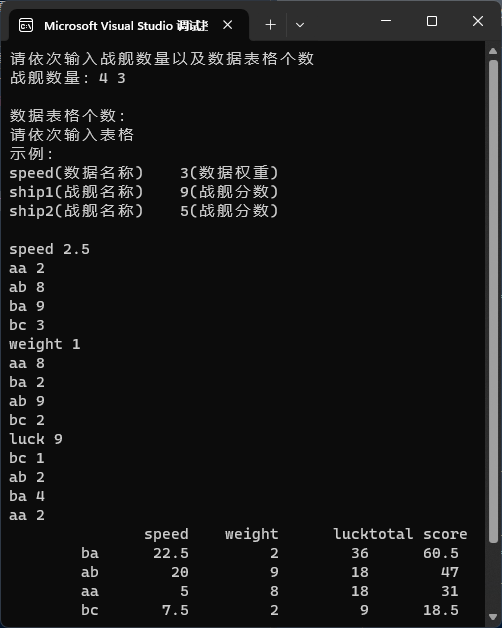
\includegraphics[scale=0.75]{pic1.png}
    \caption{测试输入及输出}
\end{figure}
